% LaTeX Boilerplate
% LaTeX Boilerplate:    Packages {{{
\documentclass{article}
\usepackage{algorithmic}
\usepackage{algorithm}
\usepackage{amsmath,amsfonts}
\usepackage{array}
\usepackage{arydshln} % for horizontal dashed lines in table
\usepackage{balance}
\usepackage{bbm}
\usepackage{chngcntr}
\usepackage{cite}
\usepackage{float}
\usepackage{gensymb} % for degrees symbol
\usepackage{graphicx}
\usepackage{listings}
\usepackage{mathtools}
\usepackage{setspace}
\usepackage{stfloats}
\usepackage{subcaption}
%\usepackage[caption=false,font=normalsize,labelfont=sf,textfont=sf]{subfig}
\usepackage{tabularx}
\usepackage{textcomp}
\usepackage{tikz}
\usepackage{titlesec}
\usetikzlibrary{calc}
\usetikzlibrary{math}
\usepackage{url}
\usepackage{verbatim}
\usepackage{xcolor}
\usepackage{hyperref}
\usepackage{cleveref}
%}}}
% LaTeX Boilerplate:    Environment Setup  {{{
\definecolor{customBlue}{RGB}{0,80,150}
\hypersetup{
   colorlinks=true,
   linkcolor=customBlue,
}
\setlength{\parindent}{0pt}
\setlength{\parskip}{0.7em}
\counterwithin{equation}{section}

\lstdefinestyle{myMatlabStyle}{
   language=Matlab,
   keywordstyle=\color{blue}\bfseries,   % Keywords are blue and bold
   commentstyle=\color{green!60!black},  % Comments are dark green
   stringstyle=\color{red},              % Strings are red
   basicstyle=\ttfamily\fontsize{6.2pt}{8pt}\selectfont,
   frame=single,
   captionpos=b                          % Caption at the bottom
}
% }}}
% Title {{{
\titleformat{\subsection}
   {\normalfont\normalsize\bfseries} % format
   {\thesubsection}                % label
   {0.8em}                           % sep
   {}                              % before-code
\titlespacing*{\subsection}
   {0pt}
   {3.5ex}
   {1.0ex}
\begin{document}
\renewcommand{\thesection}{\Alph{section}}
\begin{titlepage}
   \centering
   \vspace*{\fill}  % Pushes content to vertical center

   {\Huge\bfseries Effective Roughness Models \par}
   \vspace{1cm}

   {\Large Andrew Whelan \par}
   \vspace{0.5cm}

   {\large \date{\today} \par}

   \tableofcontents
   \vspace*{\fill}  % Pushes remaining space below
\end{titlepage}
% }}}

% TODO {{{
%\section*{TODO}
%The below derivations are not quite as nice as I'd like, however, I'm probably
%spending a little too much time on prettifying the assumptions so... here's a list of
%things to do after I've looked at the actual model comparisons and gotten some
%results (focusing on that this week):
%\begin{enumerate}
%   \item Refine the notation,
%   \item Make a glossary,
%   \item Complete the assumptions,
%   \item Come up with a sensible taxonomy of assumptions, and format appropriately
%   \item Refine the derivations so that we only number significant results,
%\end{enumerate}
%% }}}
%% TODO: revise equation numbering later on, to reflect "common" assumptions across
%% scattering models
%
%\newpage
% Notation {{{
\setcounter{section}{13} % "N"
\setcounter{subsection}{-1}
\setcounter{equation}{0}
\section{Notation}
\begin{center}
\renewcommand{\arraystretch}{1.40}
\begin{tabular}{ m{12em} m{25em} }
   $(\vec{r}, t) \in \mathbb{R}^{3+1}$ & Coordinates \\
   $\mathbf{\hat{e}} = ( \mathbf{\hat{e}}_1, \mathbf{\hat{e}}_2, \mathbf{\hat{e}}_3
      )$ & Abstract vector space basis \\
   $\Sigma_{\partial} = \{ \vec{r} \ | \ f_{\Sigma_{\partial}}(\vec{r}) = 0 \}$ &
      Boundary between two media \\
   $\Sigma_{R} = \{ \vec{r} \ | \ f_{\Sigma_{R}}(\vec{r}) = 0 \}$ &
      Surface of point-receivers \\
   $\Omega = \{ \vec{r} \ | \ f_{\Sigma_{\partial}}(\vec{r}) < 0 \}$ &
      Reflected volume \\
   $\vec{r}_T, \vec{r}_\partial, \vec{r}_R$ & Positions of transmitter, scattering
      point, and receiver \\
   $\hat{n}_{\Sigma}( \vec{r} ) = \frac{\nabla f_{\Sigma}}{|\nabla f_{\Sigma}|}$ &
      Unit surface normal along $\Sigma$ \\
   $d \vec{A}_{\Sigma}( \vec{r} ) = \hat{n}_{\Sigma} ( \vec{r} ) \ dA_{\Sigma} (
      \vec{r} )$ & Vector surface area element of $\Sigma$ \\
   $\mathcal{E}( \vec{r}, t ) = \text{Re} \{ e^{j \omega t} \mathbf{E}( \vec{r} ) \}$
      & Electric Field \\
   $\mathbf{E}( \vec{r} ) \in \mathbb{C}^3$ & Electric Field Phasor \\
   $\mathcal{H}( \vec{r}, t ) = \text{Re} \{ e^{j \omega t} \mathbf{H}( \vec{r} ) \}$
      & Magnetic Field \\
   $\mathbf{H}( \vec{r} ) \in \mathbb{C}^3$ & Magnetic Field Phasor \\
   $\vec{\mathcal{S}}(\vec{r}, t) \overset{\text{def}}{=} \mathcal{E} \times
      \mathcal{H}$ & Poynting vector \\
   $\langle \vec{\mathcal{S}} \rangle (\vec{r}) \overset{\text{def}}{=}
      \frac{\omega}{2 \pi} \int_0^{\frac{2 \pi}{\omega}} \vec{\mathcal{S}}(t) dt$ &
      Time-averaged Poynting vector \\
   $\vec{\xi}_i \overset{\text{def}}{=} ( \epsilon_i, \mu_i, \sigma_i )$ &
      Constitutive Parameters ($i$ indexes the medium) \\
   $\eta \overset{\text{def}}{=} \sqrt{ \frac{j \omega \mu}{\sigma + j \omega
      \epsilon}} \in \mathbb{C}$ & Intrinsic impedance of wave medium \\
   $\mathbf{E}(\vec{r} ) = |\mathbf{E}( \vec{r} ) | e^{j \chi_E}
      \mathbf{\hat{e}}_{\chi_E}$ & Linearly polarized $\mathbf{E}$ phase
      decomposition \\
   $\chi_E, \ \chi_H \in \mathbb{R}$ & Propagation phases \\
   $\mathbf{\hat{e}}_{\chi_E}, \ \mathbf{\hat{e}}_{\chi_H} \in \mathbb{R}^3$ & Unit
      (linear) polarization vectors \\
   $\phi \overset{\text{def}}{=} \cos^{-1}( \mathbf{\hat{e}}_{\chi_E} \cdot
      \mathbf{\hat{e}}_{\chi_H} )$ & Spatial phase \\
   $\theta_{\Sigma} \overset{\text{def}}{=} \cos^{-1} (\frac{\langle
      \vec{\mathcal{S}} \rangle \cdot \hat{n}_{\Sigma}}{|\langle \vec{\mathcal{S}}
      \rangle |})$ & Propagation angle \\
   $dP_{\Sigma}(\vec{r}) \overset{\text{def}}{=} \langle \vec{\mathcal{S}} \rangle
      \cdot d \vec{A}_{\Sigma}$ & Incremental power over $\Sigma$ \\
      $\mathcal{T}(\vec{r}) + \mathcal{R}(\vec{r}) = 1$ & Local Power Balance \\
   $\mathcal{T}(\vec{r})$ & Transmittance (portion of $dP$ transmitted through
      $\Sigma$) \\
   $\mathcal{R}(\vec{r}) = \mathcal{R}_S(\vec{r}) + \mathcal{R}_R(\vec{r})$ &
      Reflectance (portion of $dP$ reflected back) \\
   $\mathcal{R}_R(\vec{r}) = R^2 |\Gamma(\vec{r})|^2$ & Specular reflectance \\
   $\mathcal{R}_S(\vec{r}) = S^2 |\Gamma(\vec{r})|^2$ & Diffuse reflectance \\
   $\Gamma(\vec{r}) \in \mathbb{C}$ & Fresnel reflection coefficient \\
\end{tabular}
\end{center}
%  % }}}

\newpage
\setcounter{section}{0}   % Because first section is unnumbered
\setcounter{subsection}{0}
\setcounter{equation}{0}  % ```
\section{Model Assumptions}
% A.1. Scattering Parameter S {{{
\subsection{Scattering Parameter $S$}
\begin{equation}
   S \in [ 0, 1 ], \text{ is a constant parameter capturing \emph{effective
   roughness} of } \Sigma_{\partial}.
   \label{eq:erParameters}
\end{equation}
% }}}
% A.2. Transmittance is weakly dependent on Geometry {{{
\subsection{Transmittance is weakly dependent on Geometry}
\begin{equation}
   \text{We can vary $R$ and $S$ without adversely affecting } \mathcal{T}: \quad \frac{\partial \mathcal{T}}{\partial(R, S)} \approx 0
   \label{eq:transmittanceWeaklyGeometric}
\end{equation}
% }}}
% A.3. Homogeneous Scatterer {{{
\subsection{Homogeneous Scatterer}
\begin{equation}
   S^2 |\Gamma|^2 dP_{\Sigma_{\partial}} = \iint_{\Omega} I( \theta, \phi ) d \theta
      d \phi
   \label{eq:homogeneousScatter}
\end{equation}
%  % }}}
% A.3  Incoherent Scattering {{{
\subsection{Incoherent Scattering}
Scattered wave phases are random \& uncorrelated, so power sums incoherently: 
\begin{align}
   S^2 dP_{\Sigma_{R, S}} ( \vec{r} ) &\overset{\mathclap{\text{def}}}{=}
      dP_{\Sigma_R} - R^2 dP_{\Sigma_{R, GO}} \nonumber \\
   &= \int_{\Sigma_{\partial}} \left( \int_{\theta_{\Sigma_R} - \frac{d
      \theta_{\Sigma_R}}{2}}^{\theta_{\Sigma_R} + \frac{d \theta_{\Sigma_R}}{2}}
      \int_{\phi_{\Sigma_R} - \frac{d \phi_{\Sigma_R}}{2}}^{\phi_{\Sigma_R} + \frac{d
      \phi_{\Sigma_R}}{2}} I( \theta, \phi ) \ d \phi \ d \theta \right)
   \label{eq:incoherence}
\end{align}
% }}}

\setcounter{section}{5} % "F"
\setcounter{subsection}{0}
\setcounter{equation}{0}
\section{Field Assumptions}
% F.1. Remote Antennas {{{
\subsection{Remote Antennas}
Antennas are not in the near-field (an outdoor scenario), so we have
\begin{equation}
   \phi = \frac{\pi}{2}, \quad \chi_E = \chi_H
   \label{eq:remoteAntennas}
\end{equation}
%  % }}}
% F.2. Medium 1 {{{
\subsection{Medium 1}
The wave is travelling in free space until it hits an obstruction:
\begin{equation}
   (\epsilon_1, \mu_1, \sigma_1) = (\epsilon_0, \mu_0, \sigma_0).
   \label{eq:medium1}
\end{equation}
%  % }}}
% F.3. Medium 3 {{{
\subsection{Medium 2}
The obstruction is a PEC (this can be adjusted later):
\begin{equation}
   (\epsilon_2, \mu_2, \sigma_2) = (\epsilon_0, \mu_0, \infty).
   \label{eq:medium2}
\end{equation}
%  % }}}

\setcounter{section}{3}   % Because first section is unnumbered
\setcounter{subsection}{0}
\setcounter{equation}{0}  % ```
\section{Direct Consequences}
% D.1. Local Incremental Power {{{
\subsection{Local Incremental Power}
The formula for local incremental power can be simplified into two useful forms:
\begin{subequations}
\begin{align}
   dP_{\Sigma}(\vec{r}) &= \langle \vec{{\mathcal{S} }}(\vec{r}) \rangle \cdot d
      \vec{A}_{\Sigma} ( \vec{r} ) \nonumber \\
   &= \text{Re}( \mathbf{E}(\vec{r}) \times \mathbf{H}(\vec{r})^{*} ) \cdot
      \hat{\mathbf{n}}_{\Sigma}(\vec{r}) \\
   &= | \langle \vec{\mathcal{S}} \rangle | \cos( \theta_{\Sigma} )
      dA_{\Sigma} 
      \label{eq:localIncrementalPowerPoynting}
\end{align}
\end{subequations}
% }}}
% D.2. Transmittance Approximation {{{
\subsection{Transmittance Approximation}
\eqref{eq:erParameters} and \eqref{eq:transmittanceWeaklyGeometric} mean that we can
adjust $S$ and $R$ without adversely affecting $T$. So, considering the perfectly
specular case $S=0, R=1$, we get
\begin{align}
   \mathcal{T} &\approx 1 - | \Gamma |^2 \nonumber \\
   \implies R^2 + S^2 & \approx 1 
   \label{eq:RApprox}
\end{align}
%  % }}}

\renewcommand{\thesection}{\arabic{section}}
%\counterwithout{equation}{section}
\setcounter{section}{0}
\setcounter{equation}{0}
\section{2D Lambertian-Model}
Here, we have a restricted 2d setup, and assume a cylindrical wave source:
\begin{equation}
   | \langle \vec{\mathcal{S}} \rangle | = \frac{K}{|\vec{r} - \vec{r}_T|}
   \label{eq:cylindricalSourceAssumption}
\end{equation}
We can calculate $K$ by integrating over a wavefront that doesn't intersect
$\Sigma_{\partial}$:
\begin{align}
   P_0 &= \int_{0}^{2 \pi} | \langle \vec{\mathcal{S}} \rangle | dl = \int_0^{2 \pi}
      \frac{K}{|\vec{r} - \vec{r}_T|} dl \nonumber \\
   &= \int_0^{2 \pi} \frac{K}{|\vec{r} - \vec{r}_T|} |\vec{r} - \vec{r}_T| d \theta
      = 2 \pi K \nonumber \\ 
   \overset{\eqref{eq:cylindricalSourceAssumption},
      \eqref{eq:localIncrementalPowerPoynting}}{\implies} dP_{\Sigma_{\partial}} ( \vec{r} )
      &= \frac{P_0 \cos \theta_{\Sigma_{\partial}}}{2 \pi |\vec{r} - \vec{r}_T|}
      dl_{\Sigma_{\partial}} \label{eq:cylindricalSource}
\end{align}
The Lambertian scattering assumption in 2D is (see \eqref{eq:homogeneousScatter}):
\begin{align}
   I( \theta ) &= D \cos \theta  \label{eq:lambertian2dAssumption} \\
   \implies S^2 | \Gamma |^2 dP_{\Sigma_{\partial}} &=
      \int_{-\frac{\pi}{2}}^{\frac{\pi}{2}} D \cos \theta d \theta = 2D \nonumber \\
   \overset{\eqref{eq:lambertian2dAssumption}
      ,\eqref{eq:cylindricalSource}}{\implies} I( \theta ) &= \frac{S^2 |\Gamma|^2
      P_0 \cos \theta_{\Sigma_{\partial}} dl_{\Sigma_{\partial}}}{4 \pi |\vec{r} -
      \vec{r}_T|} \cos \theta \nonumber \\
   \overset{\eqref{eq:incoherence}}{\implies} dP_{\Sigma_{R, S}} &=
      \frac{1}{S^2} \int_{\Sigma_\partial} \left( \int_{\theta_{\Sigma_{R}}- \frac{d
      \theta_{\Sigma_{R}}}{2} }^{\theta_{\Sigma_{R}} + \frac{d
      \theta_{\Sigma_{R}}}{2} } \frac{P_0 S^2 |\Gamma|^2 }{4 \pi |\vec{r}_{\partial}
      - \vec{r}_T| } \cos \theta d \theta \right) \cos \theta_{\Sigma_{\partial}}
      dl_{\Sigma_{\partial}} \nonumber \\
   &= \int_{\Sigma_\partial} \left( \frac{P_0 |\Gamma|^2 \cos
      \theta_{\Sigma_{R}}}{4 \pi |\vec{r}_{\partial} - \vec{r}_T| } d
      \theta_{\Sigma_{R}} \right) \cos \theta_{\Sigma_{\partial}} dl_{\Sigma_{\partial}} \nonumber \\
   &= \frac{P_0}{4 \pi} \left( \int_{\Sigma_\partial} \frac{|\Gamma|^2 \cos
   \theta_{\Sigma_{R}} \cos \theta_{\Sigma_{\partial}} }{|\vec{r}_{\partial}
   - \vec{r}_T||\vec{r}_{R} - \vec{r}_{\partial}|} dl_{\Sigma_{\partial}} \right)
   dl_{\Sigma_R} 
\end{align}
$dP_{\Sigma, GO}$, the portion as calculated via Geometrical Optics, is given by:
\begin{equation}
   dP_{\Sigma, GO} = \mathbbm{1}_{\Sigma_\partial} (\vec{r}_{\text{spec}})
      \frac{P_0}{2 \pi} \left( \frac{|\Gamma|^2 \cos \theta_{\text{spec}}}{
      |\vec{r}_{\text{spec}} - \vec{r}_T| + |\vec{r}_R - \vec{r}_{\text{spec}}| }
      \right) dl_{\Sigma_R}
   \label{eq:GOPowerCalc}
\end{equation}

\subsection{Setup Simplifications}
Assume that the second medium is a PEC strip starting at $(w_{x0}, 0)$ and ending at
$(w_{xe}, 0)$:
\begin{equation}
   \Sigma_{\partial} = \{ (w_x, 0) \in \mathbb{R}^2 \ | \ w_x \in [ w_{x0}, w_{xe} ] \}
   \label{eq:boundaryPosition}
\end{equation}
So that
\begin{equation}
   \vec{r}_{\text{spec}} = ( w_{\text{spec}}, 0 )
   \label{eq:specPointFlatWall}
\end{equation}
The line of receivers is parallel to the strip:
\begin{equation}
   \Sigma_{R} = \{ (r_x, r_y) \in \mathbb{R}^2 \ | \ r_x \in [ r_{x0}, r_{xe} ] \}
   \label{eq:receiverPositions}
\end{equation}
The transmitter is fixed:
\begin{equation}
   \vec{r}_T = (t_x, t_y)
   \label{eq:transmitterPosition}
\end{equation}
We also assume that the source is linearly polarized with the electric field normal
to the plane of incidence, so that 
\begin{equation}
   |\Gamma|^2 = 1
   \label{eq:polarizationSimplification}
\end{equation}

We then get:
\begin{align*}
   dx &= dl_{\Sigma_{\partial}} = dl_{\Sigma_R} \\
   \frac{\cos \theta_{\Sigma_R}}{| \vec{r}_{\partial} - \vec{r}_T |} &= \frac{t_y}{t^2_y + (w_x - t_x)^2} \\
   \frac{\cos \theta_{\Sigma_{\partial}}}{| \vec{r}_{R} - \vec{r}_{\partial} |} &= \frac{r_y}{r^2_y + (r_x - w_x)^2} \\
   w_{\text{spec}} &= t_x + t_y \left( \frac{r_x - t_x}{r_y + t_y} \right) \\
   &= r_x - r_y \left( \frac{r_x - t_x}{r_y + t_y} \right) \\
   \implies \cos \theta_{\text{spec}} &= \frac{r_y + t_y}{\sqrt{(r_x - t_x)^2 +
      (r_y+t_y)^2}}, \quad \text{and} \\
   |\vec{r}_{\text{spec}} - \vec{r}_T| + |\vec{r}_R - \vec{r}_{\text{spec}}| &=
      \sqrt{(r_x - t_x)^2 + (r_y + t_y)^2}
\end{align*}

which lead to the explicit spatial power distributions along the line of receivers:
\begin{align}
   dP_{\Sigma_{R, S}} &= \frac{P_0}{4 \pi} \left( \int_{w_{x0}}^{w_{xe}} \frac{t_y
      r_y}{\left( t_y^2 + (x' - t_x)^2 \right) \left( r_y^2 + (x - x')^2 \right)}
      dx' \right) dx \label{eq:powerDistributionERScattered} \\
   dP_{\Sigma_{R, GO}} &= \frac{P_0}{4 \pi}
      \begin{dcases}
         2 \cdot \frac{t_y + r_y}{(x - t_x)^2 + (r_y + t_y)^2} dx & \text{if } w_{x0} \leq
            w_{\text{spec}} \leq w_{xe} \\
         0 & \text{otherwise}
      \end{dcases} \label{eq:powerDistributionGO}
\end{align}
\newpage
\subsection{Example Setup}
\begin{figure}[h]
   \begin{center}
      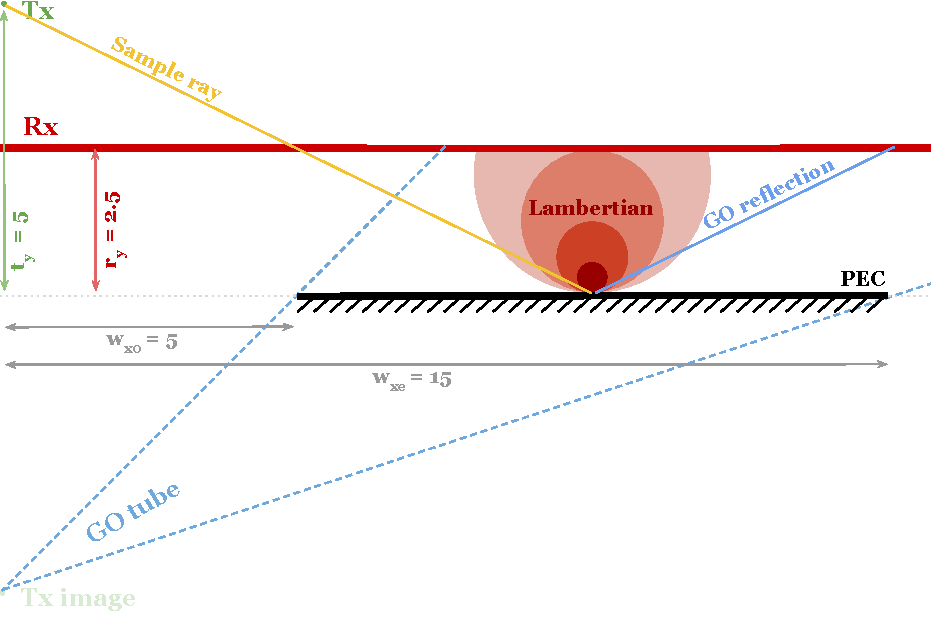
\includegraphics[width=0.75\textwidth]{../figures/Setup1.pdf}
   \end{center}
   \caption{Line of receivers and fixed point source for a PEC strip of fixed
      width}\label{fig:setup1}
\end{figure}
\begin{figure}[h]
   \begin{center}
      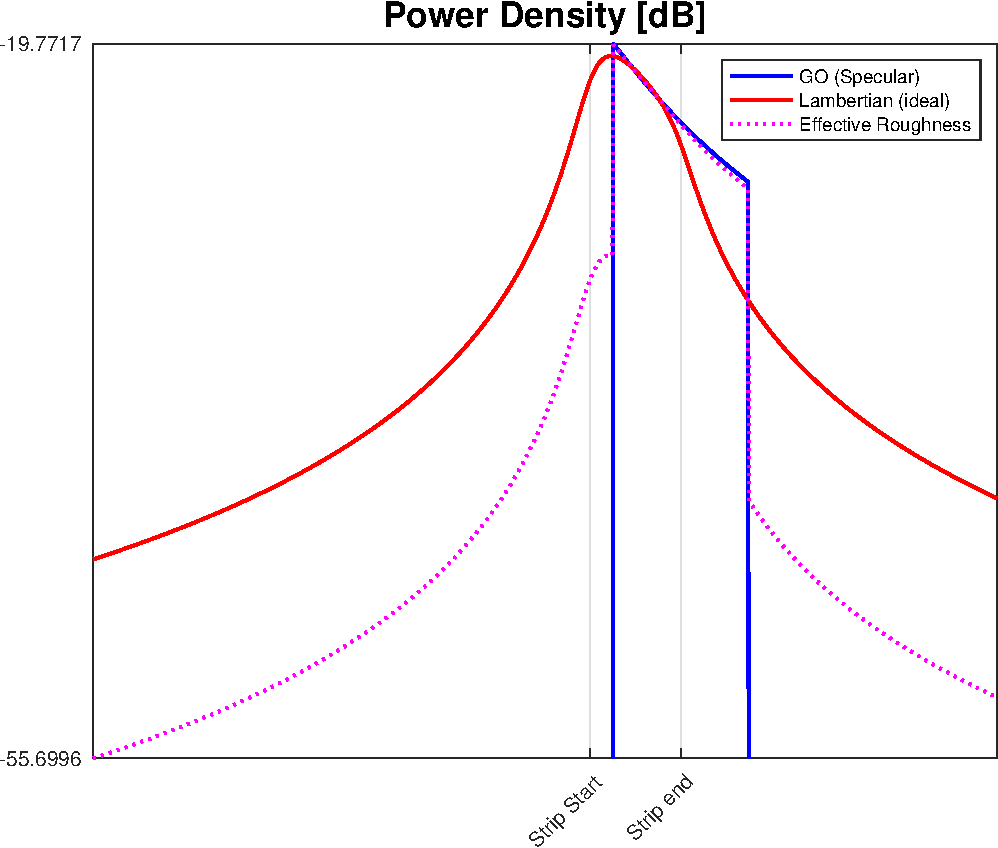
\includegraphics[width=0.55\textwidth]{../figures/PowerDensity1.pdf}
   \end{center}
   \caption{Power Density Profile for setup in \Cref{fig:setup1}.}\label{fig:PDP1}
\end{figure}
\newpage
\subsection{Lambertian Asymptotic}
A virtue of implementing the ER model is the convergence of
\eqref{eq:powerDistributionERScattered} under small values of the numerical
parameter $N_{\text{strip}}$, the number of points along the strip for the
integration, which is likely a consequence of the simple surface profile.

An even further simplification can be made, if we consider that the integrand in
\eqref{eq:powerDistributionERScattered} is the product of two Cauchy distributions,
and the whole integral, in the limit of an infinite wall, is the convolution of two
Cauchy distributions. Under this limit, we can simplify
\eqref{eq:powerDistributionERScattered} to
\begin{equation}
   dP_{\Sigma_{R,S}} \sim \frac{P_0}{4} \cdot \frac{t_y + r_y}{(x-t_x)^2 + (t_y + r_y)^2}.
   \label{eq:powerERPhysicalOptics}
\end{equation}
A comparison of \eqref{eq:powerDistributionERScattered} and
\eqref{eq:powerERPhysicalOptics} is shown in \Cref{fig:powerDensityValidation1}
(limiting case).
\subsection{Validation vs. Physical Optics Approximation}
It's instructive to compare \eqref{eq:powerDistributionERScattered} to the physical
optics case. Here, the incident electric field is given by a Hankel function:
\begin{equation}
   E^i(\vec{r}) = E_0 H_0^{(2)}(k|\vec{r} - \vec{r}_T|) \hat{\mathbf{e}}_z
   \label{eq:incidentPOSetup1}
\end{equation}
The incident magnetic field can be calculated from Maxwell's equations:
\begin{align}
   H^i( \vec{r} ) &= \frac{j}{\omega \mu_0} \nabla \times E^i(\vec{r}) \nonumber \\
   &= \frac{j}{\omega \mu_0} 
      \begin{vmatrix} 
         \partial_x & \partial_y & \partial_z \\
         0 \quad & 0 \quad & E_0 H_0^{(2)}(k|\vec{r} - \vec{r}_T|) \\
         \hat{\mathbf{e}}_x & \hat{\mathbf{e}}_y & \hat{\mathbf{e}}_z
      \end{vmatrix}
      \nonumber \\
   &= \frac{j E_0}{\omega \mu_0 } \left( \left( \partial_y ( H_0^{(2)}(k|\vec{r} -
      \vec{r}_T|)) \right) \hat{\mathbf{e}}_x - \left( \partial_x (
      H_0^{(2)}(k|\vec{r} - \vec{r}_T|)) \right) \hat{\mathbf{e}}_y \right) \nonumber
      \\
   &= - \frac{jk E_0 H_1^{(2)} (k|\vec{r} - \vec{r}_T|) }{\omega \mu_0 |\vec{r} -
      \vec{r}_T|} \left( ( y - t_y ) \hat{\mathbf{e}}_x - ( x - t_x ) \hat{\mathbf{e}}_y\right)
\end{align}
The Physical Optics surface current is then given by 
\begin{align}
   J^{PO}(\vec{r}) &= 2 \hat{n} \times H^i( \vec{r} ) = 2 \hat{\mathbf{e}}_y \times
      H^i( \vec{r} ) \nonumber \\
   &= \frac{2jk E_0 (y-t_y) H_1^{(2)} (k|\vec{r} - \vec{r}_T|) }{\omega \mu_0
      |\vec{r} - \vec{r}_T|} \hat{\mathbf{e}}_z
\end{align}
In our case $\vec{r} \in \{ \ (x , 0) \ | \ x \in (w_{x0}, w_{xe}) \ \}$, so $y = 0$.
Using this, we can find the scattered electric field:
\begin{align}
   E_S^{PO}(\vec{r}) &= \frac{k \eta_0}{4} \int_{\Sigma_{\partial}} J^{PO}(\vec{r}^{\,\prime})
      H_0^{(2)}(k |\vec{r} - \vec{r}^{\,\prime}|) dl' \nonumber \\
   &= - \frac{j k E_0 t_y }{2} \int_{\Sigma_{\partial}}
      \frac{H_1^{(2)}(k | \vec{r}^{\,\prime} - \vec{r}_T |) \ H_0^{(2)}(k |\vec{r} -
      \vec{r}^{\,\prime}|)\hat{\mathbf{e}}_z }{|\vec{r}^{\,\prime} - \vec{r}_T|} dx'
   \end{align}
Now, compute the scattered magnetic field (complex-conjugate), again from Maxwell:
\begin{align}
   {H_S^{PO}}^* &= \frac{-j}{\omega \mu_0} \left(\nabla \times E_S^{PO} \right)^* \nonumber \\
   &= - \frac{E_0 t_y}{2 \eta_0} \left( \int_{\Sigma_{\partial}}
      \frac{H_1^{(2)}(k | \vec{r}^{\,\prime} - \vec{r}_T |) \ \nabla \times (
      H_0^{(2)}(k |\vec{r} - \vec{r}^{\,\prime}|)\hat{\mathbf{e}}_z)
      }{|\vec{r}^{\,\prime} - \vec{r}_T|} dx' \right)^* \nonumber \\
   &= - \frac{k E_0 t_y}{2 \eta_0} \left( \int_{\Sigma_{\partial}} \frac{H_1^{(2)}(k |
      \vec{r}^{\,\prime} - \vec{r}_T |)H_1^{(2)}(k |\vec{r} - \vec{r}^{\,\prime}|)
      (r_y \hat{\mathbf{e}}_x + ( (x' - x) \hat{\mathbf{e}}_y))}{|\vec{r}^{\,\prime}
      - \vec{r}_T| |\vec{r} - \vec{r}^{\,\prime}|} dx' \right)^* \nonumber \\
   &= - \frac{k E_0 t_y}{2 \eta_0} \int_{\Sigma_{\partial}} \frac{H_1^{(1)}(k |
      \vec{r}^{\,\prime} - \vec{r}_T |)H_1^{(1)}(k |\vec{r} - \vec{r}^{\,\prime}|)
      (r_y \hat{\mathbf{e}}_x + ( (x' - x) \hat{\mathbf{e}}_y))}{|\vec{r}^{\,\prime}
      - \vec{r}_T| |\vec{r} - \vec{r}^{\,\prime}|} dx' \nonumber
\end{align}
From this, we get 
{ \scriptsize
\begin{align}
   dP_S^{PO} &= \frac{1}{2} \hat{\mathbf{n}} \cdot \text{Re} ( E_S^{PO} \times
   {H_S^{PO}}^*) \nonumber \\
   &= - \frac{k^2 P_0 t_y^2 r_y}{4} \nonumber \\ 
   & \text{Im} \left( \int_{\Sigma_{\partial}}
      \frac{H_1^{(1)}(k | \vec{r}_{T,\partial} |)H_1^{(1)}(k |\vec{r}_{\partial,R}|)}{|\vec{r}_{T,\partial}| |\vec{r}_{\partial,R}|} dx' \int_{\Sigma_{\partial}} \frac{H_1^{(2)}(k |
      \vec{r}_{T,\partial} |) \ H_0^{(2)}(k |\vec{r}_{\partial,R}|)\hat{\mathbf{e}}_z }{|\vec{r}_{T,\partial}|} dx'
      \right)
   \label{eq:PowerDensityPO}
\end{align}
}
\begin{figure}[h]
   \begin{center}
      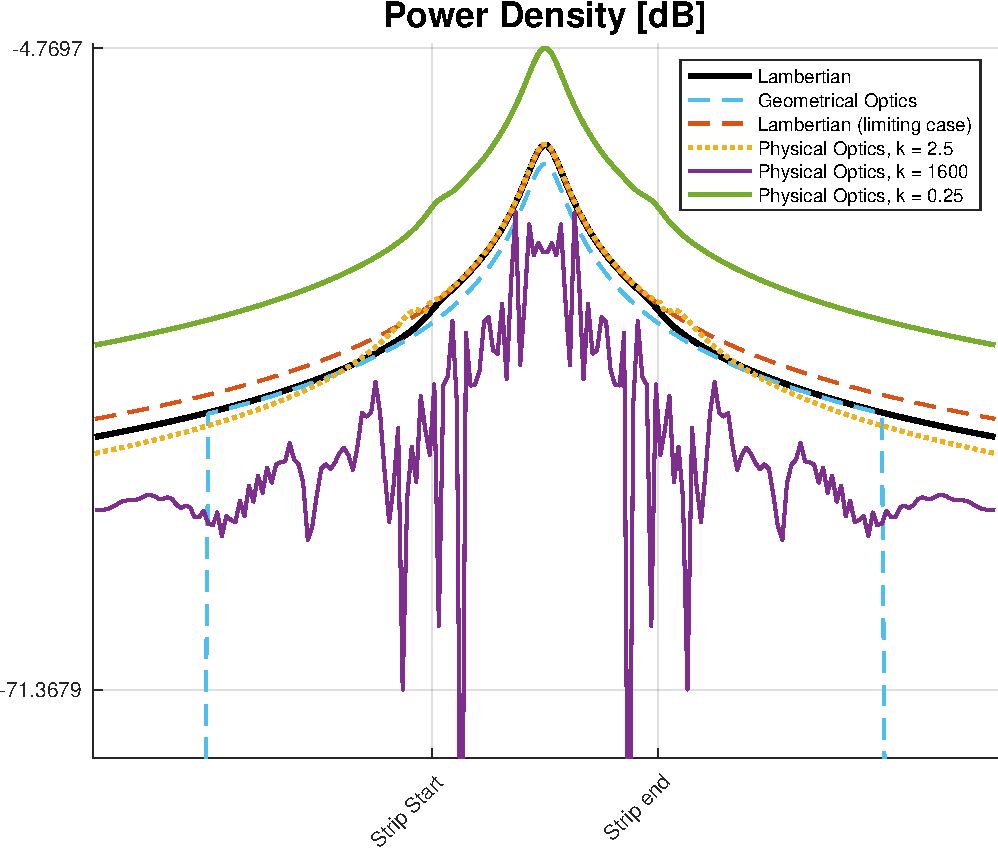
\includegraphics[width=0.75\textwidth]{../figures/PowerDensityValidation1.pdf}
   \end{center}
   \caption{Model Validation vs. Physical Optics Approximation}\label{fig:powerDensityValidation1}
\end{figure}
\newpage
\Cref{fig:powerDensityValidation1} is a revealing comparison and validation of the
models seen so far for the simple setup. Among other things, it shows that:
\begin{itemize}
   \item There is an inherent overestimation in the Lambertian models, independent of
      the scattering parameter $S$,
   \item This overestimation would likely carry over to directional models, 
   \item So, new parametric models could certainly improve the accuracy and 
      computational efficiency of the legacy models.
\end{itemize}
\subsection{Power Delay Profile}
We can also derive temporal power distributions (taking care with $t$-labels) from
\eqref{eq:powerDistributionERScattered} and \eqref{eq:powerDistributionGO} by
converting from spatial $x, x'$ coordinates to temporal $t, t'$ coordinates, via 
\begin{align}
   ct &= \sqrt{t_y^2 + (x - t_x)^2} + \sqrt{r_y^2 + (r_x - x)^2}, \quad \text{and}
      \label{eq:spaceToTimeFullPath} \\
   ct' &= \sqrt{t_y^2 + (x' - t_x)^2} \label{eq:spaceToTimePath1}
\end{align}
Inverting \eqref{eq:spaceToTimePath1} for $x'$ is a simple algebraic manipulation,
whereas \eqref{eq:spaceToTimeFullPath} inversion for $x$ requires a change of
coordinates so that the origin is at the specular point of reflection. Upon squaring
twice, the $x^4$ and $x^3$ terms then cancel.
%TODO: Show formulae for above...
\subsection{MATLAB Code}
\lstinputlisting[style=myMatlabStyle]{../matlab/PEC_1.m}
%Since we are in the far-field, the Hankel functions can be approximated: 
%\begin{align}
%   H_0^{(2)}(k|\vec{r} - \vec{r}^{\,\prime}|) & \approx ( 1 + j ) \sqrt{\frac{1}{\pi k |\vec{r} -
%      \vec{r}^{\,\prime}|}} e ^{-jk|\vec{r} - \vec{r}^{\,\prime}|}
%   \label{eq:hankelFarField} \\
%   H_1^{(2)}(k | \vec{r}^{\,\prime} - \vec{r}_T |) & \approx ( -1 + j ) \sqrt{\frac{1}{\pi k
%   |\vec{r}^{\,\prime} -
%      \vec{r}_T|}} e ^{-jk|\vec{r}^{\,\prime} - \vec{r}_T|}
%\end{align}
%leading to 
%\begin{align}
%   E_S^{PO} \approx \frac{j E_0 t_y}{\pi} \int_{\Sigma_{\partial}}
%   \frac{e^{-jk(|\vec{r}^{\,\prime} - \vec{r}_T| + |\vec{r} - \vec{r}^{
%      \,\prime}|)
%   )}}{|\vec{r}^{\,\prime} - \vec{r}_T|^{\frac{3}{2}} |\vec{r} - \vec{r}^{
%   \,\prime}|^{\frac{1}{2}}} dl' 
%\end{align}
%
%this can be used to derive the power density along the wall:
%\begin{align}
%   dP_{S}^{PO} & \approx \frac{|E_s^{PO}|^2}{2 \eta_0} \ dx \nonumber \\
%      & \approx \frac{P_0 t_y^2}{\pi^2} \left| \int_{w_{x0}}^{w_{xe}}
%      \frac{e^{-jk(\sqrt{(x')^2 + t_y^2} + \sqrt{(x - x')^2 + r_y^2}}}{((x')^2 +
%      t_y^2)^{\frac{3}{4}} ((x - x')^2 + r_y^2)^{\frac{1}{4}}} d x'
%      \right|^2 \ dx
%   \label{eq:powerPOSetup1}
%\end{align}

%\begin{align*}
%   r_s &= \sqrt{y_R^2 + (x_R - x)^2} \\
%   \cos \theta_s &= \frac{y_R}{r_s} \\
%   r_i &= \sqrt{y_T^2 + (x - x_T)^2} \\
%   \cos \theta_i &= \frac{y_T}{r_i}
%\end{align*}
%Plugging these into \eqref{eq:fieldMagEq1} we get
%\begin{equation}
%   d(|E_s|^2) = \frac{S^2 \eta_0 P_i \ y_T y_R }{2 \pi (y_R^2 + (x_R - x)^2) ( y_T^2
%      + (x - x_T)^2)} \ dx
%   \label{eq:localScaPow2dSetupParam}
%\end{equation}
%We can also express $x$ in terms of $t$ by inverting the equation
%\begin{equation}
%   (ct) = \sqrt{y_T^2 + (x - x_T)^2} + \sqrt{y_R^2 + (x_R - x)^2}
%   \label{eq:pathLength}
%\end{equation} 
%In order to invert this, we need to square twice to get rid of any square roots.
%However, in order for the $x^4$ and $x^3$ terms to cancel, we need to make a further
%coordinate transformation so the origin is at the specular point of reflection: 
%\begin{align}
%   x \to x' &= x -x_T - y_T \left( \frac{x_R - x_T}{y_R + y_T} \right) \nonumber \\ 
%   \implies x' &= x - \left( \frac{x_T y_R + x_R y_T}{y_R + y_T} \right)
%   \label{eq:coordTrans}
%\end{align}
%For the Tx term $(x - x_T)$:
%\begin{align}
%   x - x_T &= x' + \frac{y_T(x_R - x_T)}{y_R + y_T}
%\end{align}
%For the Rx term $(x_R - x)$:
%\begin{align}
%   x_R - x &= -x' + x_R - \left(\frac{x_T y_R + x_R y_T}{y_R + y_T}\right) \nonumber
%      \\
%   &= -x' + \frac{x_R(y_R+y_T) - (x_T y_R + x_R y_T)}{y_R+y_T} \nonumber \\
%   \implies x_R - x &= -x' + \frac{y_R(x_R - x_T)}{y_R + y_T}
%\end{align}
%
%Rewriting \eqref{eq:pathLength} with these new expressions:
%\begin{equation*}
%   ct = \sqrt{y_T^2 + \left(x' + \frac{y_T(x_R-x_T)}{y_R+y_T}\right)^2} + \sqrt{y_R^2
%      + \left(\frac{y_R(x_R-x_T)}{y_R+y_T} - x'\right)^2}
%\end{equation*}
%
%To simplify, define the distances from the transmitter and receiver to the specular
%point on the surface:
%\begin{align*}
%   R_{T0} &:= \sqrt{y_T^2 + \left(\frac{y_T(x_R-x_T)}{y_R+y_T}\right)^2} \\
%   R_{R0} &:= \sqrt{y_R^2 + \left(\frac{y_R(x_R-x_T)}{y_R+y_T}\right)^2}
%\end{align*}
%We then get 
%\begin{equation*}
%   ct = \sqrt{R_{T0}^2 + 2x' \frac{y_T(x_R-x_T)}{y_R+y_T} + (x')^2} + \sqrt{R_{R0}^2
%      - 2x' \frac{y_R(x_R-x_T)}{y_R+y_T} + (x')^2}
%\end{equation*}
%
%Isolate the second square root and square both sides:
%\begin{align*}
%   &(ct)^2 - 2ct \sqrt{R_{T0}^2 + 2x' \frac{y_T(x_R-x_T)}{y_R+y_T} + (x')^2} +
%      \left(R_{T0}^2 + 2x' \frac{y_T(x_R-x_T)}{y_R+y_T} + (x')^2\right) \\
%   &= R_{R0}^2 - 2x' \frac{y_R(x_R-x_T)}{y_R+y_T} + (x')^2
%\end{align*}
%
%Now collect terms and cancel:
%\begin{align*}
%   2x'(x_R-x_T) + (ct)^2 + R_{T0}^2 - R_{R0}^2 &= 2ct \sqrt{R_{T0}^2 + 2x'
%      \frac{y_T(x_R-x_T)}{y_R+y_T} + (x')^2}
%\end{align*}
%
%Squaring both sides: 
%\begin{align*}
%   &4\left( (x_R - x_T)^2 + (ct)^2 \right)^2 (x')^2 + \\
%   &4(x_R - x_T) \left( R_{T0}^2 - R_{R0}^2 + (ct)^2 \left( \frac{y_R - y_T}{y_R +
%      y_T} \right) \right) x' + \\ 
%   & \left( (ct)^2 + R_{T0}^2 - R_{R0}^2 \right)^2 - 4(ct)^2 R_{T0}^2
%\end{align*}
%
%Finally, we can solve for $x$ :
%\begin{align} 
%   x &= \frac{x_T y_R + x_R y_T}{y_R + y_T} - \frac{b}{2a} \pm \frac{\sqrt{b^2 -
%      4ad}}{2a}, \ \text{where} \\
%   a &= 4\left( (x_R - x_T)^2 + (ct)^2 \right)^2 \nonumber \\
%   b &= 4(x_R - x_T) \left( R_{T0}^2 - R_{R0}^2 + (ct)^2 \left( \frac{y_R - y_T}{y_R +
%      y_T} \right) \right), \nonumber \\
%   d &= \left( (ct)^2 + R_{T0}^2 - R_{R0}^2 \right)^2 - 4(ct)^2 R_{T0}^2 \nonumber \\
%   R^2_{T0} &= y_T^2 + \left(\frac{y_T(x_R-x_T)}{y_R+y_T}\right)^2, \ \text{and}
%      \nonumber \\ 
%   R^2_{R0} &= y_R^2 + \left(\frac{y_R(x_R-x_T)}{y_R+y_T}\right)^2 \nonumber
%\end{align}
%\newpage
%\section{Plane Wave Incident on PEC}
%\subsection{Questions for Conor for Fri 20 Jun 2025}
%\begin{enumerate}
%   \item Discussion of the above work, any thoughts on further refinements apart from
%      what I've listed already in the TODO section (I've spent too long on this part
%      but it will be nice to have for a writeup. I'm going to focus on the MATLAB
%      code now)?
%   \item In the above I've done the derivation for the power assuming a cylindrical
%      incoming wave. However, in the original MATLAB code setup you seem to have
%      assumed the Tx is in the far-region (hence a plane wave approximation). Do you
%      think it's sensible to adjust the above from \eqref{eq:fieldPre} for $|E_i|$?
%   \item What measures specifically do you think would be good to compare first? I
%      think last time you mentioned the power profiles as a first step. So, do you
%      think calibrating the model correctly 
%\end{enumerate}
\end{document}
% Bibliography {{{
\bibliographystyle{IEEEtran}
\bibliography{refs}
\end{document}
%}}}
